\documentclass[journal]{IEEEtran}
\usepackage{blindtext}
\usepackage{graphicx}
\usepackage[none]{hyphenat}
\usepackage{minted}
\usepackage[dvipsnames]{xcolor}

\definecolor{LightGray}{HTML}{F9F9F9}

\setminted{breaklines=true}
\usemintedstyle{monokailight}

\begin{document}
\title{Android Performance Analysis and \\ Optimization Techniques}

\author{Areeb Jamal and Divya Prakash Varshney \\
	 \IEEEmembership{Computer Engineering 3rd Year, ZHCET}}

% The paper headers
\markboth{Android Optimization Techniques, April~2016}%
{Android Performance}


% make the title area
\maketitle


\begin{abstract}
Android, being the most widely used operating system in the world, has attracted a large number of developers throughout the world. And since, the official programming language used to develop Android Apps is Java, the developers coming from its background often make wrong assumptions about the best practices in Android. Making these apps perform poorly in respect to CPU and memory utilisation. The purpose of this paper is to discuss some common solutions to optimization problems associated with Android.
\end{abstract}


\section{Introduction}
There are 3 areas of performance in mobile computing :
\begin{itemize}
	\item CPU
	\item Memory
	\item Network
\end{itemize}
Because of the fact that \emph{Network} optimization is generally language agnostic and is covered in various modern netwroking libraries, we will focus on \emph{CPU} and \emph{Memory} usage optimization and analysis techniques.\\
The CPU utilization in case of mobile computing can be closely tied to memory as poor RAM optimisation may lead to repeated calls of Garbage Collector leading to wasteful CPU cycles meaning frame rate drops, so in order to optimize CPU performance, we should also improve the memory usage of the application.

\section{Need of Performance}
The need to optimize performance of any application comes from a basic need of user to avoid using applications that lag through the common workflow.\\
To ensure smooth performance, app needs to call the basic \emph{onDraw()} function 60 times a second, leading to the 60 FPS mark of GPU rendering. Any operation that reduces the number of calls of this function leads to detrimental performance. The reason of this frame rate drop can be anything that keeps CPU busy and thus unable to call \emph{onDraw()} enough times.\\
Also, Android emplys a \emph{Low Memory Killer (LMK)} which kills backround applications according to memory they are using, meaning the better memory optimization we use, more time our app gets to live in background.\\
We will now enumerate the reasons why an Android application lags

\newpage

\subsection{Heavy Computations or Network Calls}
Heavy Computations or Network Calls \emph{(like downloading images, making API calls, etc)} when done on Main Thread \emph{(known as UI thread in Android)}, lead to wasteful CPU cycles which could be used to render UI. These computations can emulate \emph{blocking} or \emph{busy waiting} and thus should be moved to another \emph{Thread} of their own.\\
A further improvement can be made by caching the frequently made calculations, removing the need of using threads. Caching does not necessarily improve performance but decreases the waiting time for the user as concurrency ensures no frame rate drops but still takes the same amount of time in calculating the results.\\
Since it is a well known solution \emph{(yet developers tend to ignore)}, we will not discuss it any further.

\subsection{Repeated GC Calls}
Another reason developers forget to consider is that the Android runtime invokes Garbage Collector every time it needs to replenish the memory as it feels the free RAM is getting less. If there are huge memory allocations in the application, GC call frequency will be considerably increased and thus frame rates will drop leading to lag.\\
Common solution to this problem is using better data structures specific to Android, usually not consistent with the Java Development Guidlines, as it focuses on general development.

\subsection{Memory Leaks}
A severe case of repeated GC calls take place if there is a memory leak. Because GC cannot reclaim memory on each run, Android Runtime continues invoking it until a minimum amount of free RAM is ensured. With a memory leak, this won't be able to happen and thus, GC will run more frequently, increasing the memory consumed by our and and also decreasing its performance.

\newpage

\section{Analysis and Solutions}
In further sections, we will discuss the topics we analysed and provide solutions to those specific problems in context of Android Development

\subsection{Memory Leaks}
Major portion of our analysis has been on memory leaks and to provide better solutions to ensure they don't happen. We will start by defining a memory leak.\\

\begin{center}
	DEFINITION
\end{center}
A memory leak \cite{memleak}, in Object Oriented Programming, happens when an object is not needed in program anymore and still resides in memory. And hence, program may never be able to reference it again and so has no way of knowing that some leaked objects are consuming resources and impacting performance.\\
Since objects are removed from memory using Garbage Collector, they are not derefenced immediately. Instead, a programmer is advised to let GC work in background to remove unused objects, hence taking control from programmer to release this memory. However it is convenient from implementation point of view, it makes memory leaks very hard to debug and easy to occur.\\

Memory Leaks are in Android are usually related to objects bound by a particular lifecycle. When they are kept in memory after their lifecycle has completed, it is usually considered a memory leak. Any Android Developer will know that an \emph{Activity} is a standard Android View class with associated lifecycle. So, if an Activity is instructed by the system to be destroyed and it can't because it is referenced somewhere is a memory leak condition.\\

Usually, developers pass their activity instances wherever a \emph{Context} argument is needed and if that instance is held on by any other object, the Acitivity will reside in memory till that reference is not cleared. And since the Activity is likely to be destroyed if it needs to be garbage collected, means it completed it lifecycle leaving no control to the developer to clear that reference, creating a somewhat deadlock kind of situation of memry leak where it never gets resolved.\\

\begin{center}
	COMMON MEMORY LEAKS
\end{center}

Some common memory leak examples in Android are :\\

\begin{itemize}
	\item \emph{Static Context Leak}\\
	A reference held by a static variable has lifetime of entire application, and hence can't be removed until the app closes, meaning if an Activity reference is stored in a static variable, Garbage Collector won't be able to remove the instance of memory, causing a memory leak. This is naturally the easiest way \cite{ways} to cause one and is widespread throughout codes of Android Developers.
	
	\newpage
	
	The same applies if any Context subclass is stored in a static variable, namely:
	\begin{itemize}
		\item Activity
		\item View
		\item Service
	\end{itemize}
\begin{minted}[bgcolor=LightGray]{Java}
private static Context context;
	
@Override
  public void onCreate(Bundle save) {
  context = this;
}
\end{minted}

	\item \emph{Non Static Inner Classes}\\
	The non static Inner Class always holds a reference to the outer class, and if this class is a Context subclass, then there is an eminent memry leak as each instance of such inner class will hold a reference to outer class and will be independent of Activity Lifecycle, making it difficult for GC to collect the activity if inner class still holds a reference to it.\\
	
	If the original Activity is replaced by another one, the inner class reference will be in invalid state, and can result in application crash as well.
\begin{minted}[bgcolor=LightGray]{Java}
public void onCreate(Bundle save) {
  /* ... */
  btn.setOnClickListener((view) -> {
    (new DummyClass()).doSomeTask();
  });
}

class DummyClass {
  public void doSomeTask() {
    /* Some Task */
  }
}
\end{minted}
\\

	\item \emph{Anonymous Classes}\\
	The same effect will occur if an anonymous class is declared in a context subclass such as Activity, as it also holds a reference to containing class. More detrimental effect will happen if a asynchronous task is executed in such a way. Because if it continues to perform background work after the Activity has been destroyed, the reference to the Activity will persist and it won’t be garbage collected until after the background task completes.\\
	
	\newpage
\begin{minted}[bgcolor=LightGray]{Java}
void downloadImage() {
  new AsyncTask<...>() {
    @Override
    protected Void doInBackground(Void... params) {
      /* Download Image */
      return image;
    }
    
    @Override
    protected Void onPostExecute(Image image) {
      imageView.setBackground(image);
    }
    
  }.execute();
}

public void onCreate(Bundle save) {
  /* ... */
  btn.setOnClickListener((view) -> {
    (new DummyClass()).doSomeTask();
  });
}
\end{minted}
	In case the activity is replaced by another one, like when orientation is changed, the AsyncTask will not be destroyed and continue running, hence keeping the original activity in memory and once it finishes, it will try to update the views which are replaced already with another Activity, thus potentially causing a crash by NullPointerException
	
	This example being an extension of previous is very different use case and can present a memory leak in various deiiferent contexts but with similar pattern.
	\begin{itemize}
		\item Handlers
		\item Threads
		\item Listeners
		\item TimerTasks
		\item Sensor Managers\\
	\end{itemize}
	

\end{itemize}

\begin{figure}[h]
	\centering
	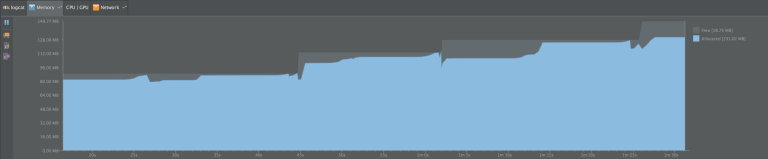
\includegraphics[width=0.7\linewidth]{memleak}
	\caption[]{Memory usage of Memory Leaked App \cite{fixing}}
	\label{fig:memleak}
\end{figure}

\begin{figure}[h]
	\centering
	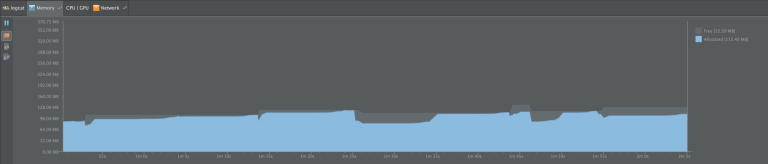
\includegraphics[width=0.7\linewidth]{nomemleak}
	\caption[]{Normal memory usage of same app \cite{fixing}}
	\label{fig:nomemleak}
\end{figure}

\newpage

\begin{center}
	SOLUTIONS
\end{center}

\subsection{ArrayList Optimizations}
ArrayList is the most commonly used implementation of List Collection in Java SDK, used to store arrays data of same type. ArrayList in java has default memory size of 8, but Android SDK initializes ArrayList with size 0 by default.When any data is added to ArrayList, it first checks if the size of ArrayList is sufficient enough to  the data, and if so, it adds the data but in case where the size isn't enough to accomodate it, then ArrayList allocates a new memory with larger size (in multiples of 8), copies all the previously stored data in new memory, remove old memory used and finally add the new data.

\emph{For example :} If there are 1000 objects to be stored in ArrayList and objects are added one by one, then after each multiple of 8 items, new memory will be allocated about $\log_8(1000)$ times.

The allocation of memory repeatedly, and copying the data from previous location to new wastes enough amount of time. Also if the object's size is huge, then copying even single data object my take a significant amount of time in loops.

A better approach would be intializing arraylist with the data size for example :

\begin{minted}[bgcolor=LightGray]{Java}
public List<String> getStudents(List<Student> students){
  List<String> student = new ArrayList<>(students.size());
  for (Student s : students){
    student.add(s.name);
  }
  return student;
}
\end{minted}
This will allocate the memory only once and lot of time will be saved in allocating and copying
the data. Even if this memory is insufficient, only few excess memory allocations will take place.


\subsection{Enums vs Static Constants}
Whenever we need to define states for an object or any other use case, we use Enums. Enums are classes which have their own variable and can also have their own methods. Since they act like classes, there is an associated memory overhead. Although Enums can help in type safety, their use in Android causes a memory overhead which outweighs its benefits.

\emph{For example :} If a simple enum is instatiated, it has 500 bytes of memory overhead by default and if somehow we forget to make them static, then every object would have its own reference of enums and can cause lot of memory wastage.

A better approach to this problem would be using static final constants which will require lot less memory than enums and fulfill almost same work as enums.

\begin{itemize}
	\item Enums
\begin{minted}[bgcolor=LightGray]{Java}
public static enum State {
  int ON =  1;
  int OFF = 0;
};
\end{minted}
	\item Static Constants
\begin{minted}[bgcolor=LightGray]{Java}
static final int ON =  1;
static final int OFF = 0;
\end{minted}
\end{itemize}

\newpage

\subsection{StringBuilder Optimizations}
In the previous section, we talked about ArrayList, and the allocations which take place on repeated insertions. The allocations in case of StringBuilder are worse as instead of allocating in multiples, it assigns the memory exactly to the size of string needed to append + 1. Everytime a string is appended in StringBuilder, a new memory is allocated with size of previous allocated memory + new String liength +1.\\
Consider an example where you need to append 1000 names in a single string using StringBuilder. It would take 1000 allocation of memory and every time it allocate the memory the previous memory is copied into new one wasting a lot of CPU cycles.
\begin{minted}[bgcolor=LightGray]{Java}
public String getNames(List<Student> students){
  StringBuilder sb = new StringBuilder();
  for (Student s : students){
    sb.append(s.name + " ");
  }
  return sb.toString();
}
\end{minted}
A simple solution to this problem is using some random number (let's say 20) and intialize the StringBuilder with averageNumber * number of strings to be appended. This will allow to allocate the StringBuilder a starting memory and can help in reducing the allocations and CPU utilisation.
\begin{minted}[bgcolor=LightGray]{Java}
public getNames(List<Student> students){
  int num = 20;
  StringBuilder sb = new StringBuilder(num*student.size());
  for (Student s : students){
    sb.append(s.name + " ");
  }
  return sb.toString();
}
\end{minted}
Some more optimization use case for StringBuilder exist where due to lack of knowledge of certain metjods, developers succumb to bad practices in general. Take this example, this code is something whixh is very commonly seen -
\begin{minted}[bgcolor=LightGray]{Java}
for (int i = 0; i < someValue; i++){
  StringBuilder sb = new StringBuilder();
  sb.append("someConstantString");
  sb.append("someConstantString");
  sb.append(i);
}
\end{minted}
This code makes new StringBuilders repeatedly, whereas the sole purpose of StringBuilders is to maintain memory efficient append String container. To optimize this code - 
\begin{minted}[bgcolor=LightGray]{Java}
StringBuilder sb = new StringBuilder(someConstantString)
   .append(someConstantString);
int lengthOfString = sb.length();
for (int i = 0; i < someValue; i++){
  sb.append(i);
  sb.setLength(lengthOfString);
}
\end{minted}
Now this code utilizes single StringBuilder and saves the work of Garbage Collector including the time in allocation and appending of sameConstantStrong repeatedly.

\subsection{SpareArray vs HashMap}
\emph{SparseArray}s \cite{sparsearray} are memory efficient alternatives of \emph{HashMap} (provided only in Android SDK). SparseArrays are used to map the primitive data to another set of data and has the array data structure to store keys rather than AVL tree implementation in HashMaps. What makes SparseArray memory efficient than the HashMap is use of primitive data type as keys removing the need of autoboxing Objects to primitives and vice versa. Also, allocation of the primitive type takes less memory than using Object type. Another reason of its efficiency efficient is that when any key is delete from the SparseArray, instead of actually deleting the key and compacting the array; it marks the index as deleted. This entry can be used again for same key or can be collected by single garbage collection for various marked key at once, hence removing repeated GC calls on the main thread.

But SparseArrays come at the price of computational efficiency as more amount of time is needed to extract an item from SparseArray than a HashMap. So, if the use case of hashing is important, SparseArrays are obsolete in that case.

\subsection{Iterators}
Consider this code for example:
\begin{minted}[bgcolor=LightGray]{Java}
for(Event event : events) {
  /* Do some operation */
}}
\end{minted}

Java Documentation recommends that \textit{foreach} loops are the preferred way of walking through a Collection, but let us look how that translates into -
\begin{minted}[bgcolor=LightGray]{Java}
for(Event = null, Iterator it = events.iterator(); it.hasNext(); event = it.next()) {
  /* Do some operation */
}
\end{minted}
As you can see, there are many object allocations throughout the code, so calling it inside the frequent funtions like \textit{onDraw()} will be detrimental to the performance of the application and hence, rather than using iterators or foreach loop, we should use indexing. In fact, only array foreach loop runs as efficiently as indexing because Java automatically converts it to indexed loop, because arrays don't have iterators.

Here's the indexed traversal of a list -
\begin{minted}[bgcolor=LightGray]{Java}
int i = 0;
for (i; i < someList.size(); i++){
  int x = someList.size() * 3.14 / (i+1);
  Item item = someList.get(i);
  /* Do some operation */
} 
\end{minted}
An obvious problem almost every developer makes in above code is that it is calling \textit{size()} method repeatedly over the whole traversal where mostly, the colection's size never changes. A better version of the above code would be - 
\begin{minted}[bgcolor=LightGray]{Java}
int size = someList.size();
int value  = size * 3.14;
for (int i = 0; i< size; i++){
  int x = value/(i+1);
  Item item = someList.get(i);
  /* Do some operation */	
}
\end{minted}
Here, we save ourselves from repeated function calls by just storing the size in a variable

\section{Conclusion}
Android Performance Practices are easy to forget and thus cause a huge negative traction toward the developer community and Java, whereas there are easy fixes and precautions developers can take while developing their applications like not delegating resource management on Garbage Collector, handling resources themselves, using better and memory efficient data structures and tying every threaded task to the view/activity lifecycle. There are various resources detailing the process of performance optimation along with the ofiicial Android Developer Site, where developers should pay attention to those points, as Performance Matters.

\begin{thebibliography}{1}

\bibitem{}
Yoonsik Cheon, \emph{Are Java Programming Best Practices Also Best Practices for Android?}, The University of Texas at El Paso, USA

\bibitem{}
Prajakta Gotarane and Sumedh Pundkar, \emph{Smart Coding using New Code Optimization Techniques in Java to Reduce Runtime Overhead of Java Compiler}, UMIT, SNDT Womens University, Santacruz, Mumbai

\bibitem{}
Hyeon-Ju Yoon, \emph{A Study on the Performance of Android Platform}, Department of Computer Engineering, Kumoh National Institute of Technology, Gumi, Republic of Korea 

\bibitem{}
J. Bloch, Effective Java, second edition, Addison-Wesley, 2008.

\bibitem{}
Jake Wharton, \emph{Hidden Java Costs}

\bibitem{}
Best Practice for Performance,\\
https://developer.android.com/training/best-performance.html 

\bibitem{}
Huu Hai Nguyen and Martin Rinard, \emph{Detecting and Eliminating Memory Leaks Using Cyclic Memory Allocation}, Department of Electrical Engineering and Computer Science, 
Computer Science and Artificial Intelligence Laboratory, 
Singapore-MIT Alliance, 
Massachusetts Institute of Technology

\bibitem{memleak}
Memory Leak,\\
https://en.wikipedia.org/wiki/Memory-leak

\bibitem{ways}
Ways to Memory Leak in Android,\\
http://blog.nimbledroid.com/2016/05/23/memory-leaks.html

\bibitem{fixing}
Fixing Memory Leaks in Android\\
https://riggaroo.co.za/fixing-memory-leaks-in-android-outofmemoryerror/

\bibitem{sparsearray}
SparseArray\\
https://developer.android.com/reference/android/util/SparseArray.html

\end{thebibliography}

\end{document}


